\documentclass[11pt,]{article}
\usepackage{lmodern}
\usepackage{amssymb,amsmath}
\usepackage{ifxetex,ifluatex}
\usepackage{fixltx2e} % provides \textsubscript
\ifnum 0\ifxetex 1\fi\ifluatex 1\fi=0 % if pdftex
  \usepackage[T1]{fontenc}
  \usepackage[utf8]{inputenc}
\else % if luatex or xelatex
  \ifxetex
    \usepackage{mathspec}
  \else
    \usepackage{fontspec}
  \fi
  \defaultfontfeatures{Ligatures=TeX,Scale=MatchLowercase}
  \newcommand{\euro}{€}
    \setmainfont[]{IPAPMincho}
    \setsansfont[]{IPAPGothic}
\fi
% use upquote if available, for straight quotes in verbatim environments
\IfFileExists{upquote.sty}{\usepackage{upquote}}{}
% use microtype if available
\IfFileExists{microtype.sty}{%
\usepackage{microtype}
\UseMicrotypeSet[protrusion]{basicmath} % disable protrusion for tt fonts
}{}
\usepackage[margin=1in]{geometry}
\usepackage{hyperref}
\PassOptionsToPackage{usenames,dvipsnames}{color} % color is loaded by hyperref
\hypersetup{unicode=true,
            pdftitle={平成28年度社会医学実習 公衆衛生学担当分},
            pdfauthor={王 超辰},
            colorlinks=true,
            linkcolor=blue,
            citecolor=Blue,
            urlcolor=Blue,
            breaklinks=true}
\urlstyle{same}  % don't use monospace font for urls
\usepackage{color}
\usepackage{fancyvrb}
\newcommand{\VerbBar}{|}
\newcommand{\VERB}{\Verb[commandchars=\\\{\}]}
\DefineVerbatimEnvironment{Highlighting}{Verbatim}{commandchars=\\\{\}}
% Add ',fontsize=\small' for more characters per line
\usepackage{framed}
\definecolor{shadecolor}{RGB}{248,248,248}
\newenvironment{Shaded}{\begin{snugshade}}{\end{snugshade}}
\newcommand{\KeywordTok}[1]{\textcolor[rgb]{0.13,0.29,0.53}{\textbf{{#1}}}}
\newcommand{\DataTypeTok}[1]{\textcolor[rgb]{0.13,0.29,0.53}{{#1}}}
\newcommand{\DecValTok}[1]{\textcolor[rgb]{0.00,0.00,0.81}{{#1}}}
\newcommand{\BaseNTok}[1]{\textcolor[rgb]{0.00,0.00,0.81}{{#1}}}
\newcommand{\FloatTok}[1]{\textcolor[rgb]{0.00,0.00,0.81}{{#1}}}
\newcommand{\ConstantTok}[1]{\textcolor[rgb]{0.00,0.00,0.00}{{#1}}}
\newcommand{\CharTok}[1]{\textcolor[rgb]{0.31,0.60,0.02}{{#1}}}
\newcommand{\SpecialCharTok}[1]{\textcolor[rgb]{0.00,0.00,0.00}{{#1}}}
\newcommand{\StringTok}[1]{\textcolor[rgb]{0.31,0.60,0.02}{{#1}}}
\newcommand{\VerbatimStringTok}[1]{\textcolor[rgb]{0.31,0.60,0.02}{{#1}}}
\newcommand{\SpecialStringTok}[1]{\textcolor[rgb]{0.31,0.60,0.02}{{#1}}}
\newcommand{\ImportTok}[1]{{#1}}
\newcommand{\CommentTok}[1]{\textcolor[rgb]{0.56,0.35,0.01}{\textit{{#1}}}}
\newcommand{\DocumentationTok}[1]{\textcolor[rgb]{0.56,0.35,0.01}{\textbf{\textit{{#1}}}}}
\newcommand{\AnnotationTok}[1]{\textcolor[rgb]{0.56,0.35,0.01}{\textbf{\textit{{#1}}}}}
\newcommand{\CommentVarTok}[1]{\textcolor[rgb]{0.56,0.35,0.01}{\textbf{\textit{{#1}}}}}
\newcommand{\OtherTok}[1]{\textcolor[rgb]{0.56,0.35,0.01}{{#1}}}
\newcommand{\FunctionTok}[1]{\textcolor[rgb]{0.00,0.00,0.00}{{#1}}}
\newcommand{\VariableTok}[1]{\textcolor[rgb]{0.00,0.00,0.00}{{#1}}}
\newcommand{\ControlFlowTok}[1]{\textcolor[rgb]{0.13,0.29,0.53}{\textbf{{#1}}}}
\newcommand{\OperatorTok}[1]{\textcolor[rgb]{0.81,0.36,0.00}{\textbf{{#1}}}}
\newcommand{\BuiltInTok}[1]{{#1}}
\newcommand{\ExtensionTok}[1]{{#1}}
\newcommand{\PreprocessorTok}[1]{\textcolor[rgb]{0.56,0.35,0.01}{\textit{{#1}}}}
\newcommand{\AttributeTok}[1]{\textcolor[rgb]{0.77,0.63,0.00}{{#1}}}
\newcommand{\RegionMarkerTok}[1]{{#1}}
\newcommand{\InformationTok}[1]{\textcolor[rgb]{0.56,0.35,0.01}{\textbf{\textit{{#1}}}}}
\newcommand{\WarningTok}[1]{\textcolor[rgb]{0.56,0.35,0.01}{\textbf{\textit{{#1}}}}}
\newcommand{\AlertTok}[1]{\textcolor[rgb]{0.94,0.16,0.16}{{#1}}}
\newcommand{\ErrorTok}[1]{\textcolor[rgb]{0.64,0.00,0.00}{\textbf{{#1}}}}
\newcommand{\NormalTok}[1]{{#1}}
\usepackage{graphicx,grffile}
\makeatletter
\def\maxwidth{\ifdim\Gin@nat@width>\linewidth\linewidth\else\Gin@nat@width\fi}
\def\maxheight{\ifdim\Gin@nat@height>\textheight\textheight\else\Gin@nat@height\fi}
\makeatother
% Scale images if necessary, so that they will not overflow the page
% margins by default, and it is still possible to overwrite the defaults
% using explicit options in \includegraphics[width, height, ...]{}
\setkeys{Gin}{width=\maxwidth,height=\maxheight,keepaspectratio}
\setlength{\parindent}{0pt}
\setlength{\parskip}{6pt plus 2pt minus 1pt}
\setlength{\emergencystretch}{3em}  % prevent overfull lines
\providecommand{\tightlist}{%
  \setlength{\itemsep}{0pt}\setlength{\parskip}{0pt}}
\setcounter{secnumdepth}{5}

%%% Use protect on footnotes to avoid problems with footnotes in titles
\let\rmarkdownfootnote\footnote%
\def\footnote{\protect\rmarkdownfootnote}

%%% Change title format to be more compact
\usepackage{titling}

% Create subtitle command for use in maketitle
\newcommand{\subtitle}[1]{
  \posttitle{
    \begin{center}\large#1\end{center}
    }
}

\setlength{\droptitle}{-2em}
  \title{平成28年度社会医学実習 公衆衛生学担当分}
  \pretitle{\vspace{\droptitle}\centering\huge}
  \posttitle{\par}
  \author{王 超辰}
  \preauthor{\centering\large\emph}
  \postauthor{\par}
  \predate{\centering\large\emph}
  \postdate{\par}
  \date{2016年6月23日}


\usepackage{xltxtra}
\XeTeXlinebreaklocale ``ja''
\XeTeXlinebreakskip=0pt plus 1pt
\XeTeXlinebreakpenalty=0

% Redefines (sub)paragraphs to behave more like sections
\ifx\paragraph\undefined\else
\let\oldparagraph\paragraph
\renewcommand{\paragraph}[1]{\oldparagraph{#1}\mbox{}}
\fi
\ifx\subparagraph\undefined\else
\let\oldsubparagraph\subparagraph
\renewcommand{\subparagraph}[1]{\oldsubparagraph{#1}\mbox{}}
\fi

\begin{document}
\maketitle

\section{がんの記述疫学:}

\subsection{目的:}

年齢,出生コート,時期効果に関する内容を理解する.

\subsection{方法:}

日本のがん登録データをダウロードして.配布された資料を参考した上で,次の各部位のがんを解析する.各部位がんデータから年齢・出生コホート・時期効果があるかを説明する.

\subsection{課題:}

\begin{enumerate}
\def\labelenumi{\arabic{enumi}.}
\item
  肝がん死亡データの年齢,出生コホート,時期効果分析 (Group 1)
\item
  胃がん死亡データの年齢,出生コホート,時期効果分析 (Group 2)
\item
  胆のうがん死亡データの年齢,出生コホート,時期効果分析 (Group 3)
\item
  膵がん死亡データの年齢,出生コホート,時期効果分析 (Group 4)
\item
  食道がん死亡データの年齢,出生コホート,時期効果分析 (Group 5)
\item
  肺がん死亡データの年齢,出生コホート,時期効果分析 (Group 6)
\end{enumerate}

\section{参考:}

\begin{enumerate}
\def\labelenumi{\arabic{enumi}.}
\item
  \url{https://rpubs.com/kaz_yos/epi-cross-long}
\item
  配布した資料 {[}1{]} Chapter 1: 1.2 (Page 4-14)
\item
  データ入手先:cancer\_mortality(1958-2014).xls {[}2{]}
  \url{http://ganjoho.jp/reg_stat/statistics/dl/index.html}
\end{enumerate}

\section{年齢,出生コホート,時期効果に関する内容の理解}

\begin{itemize}
\tightlist
\item
  年齢効果:\\
  年齢の増加とともに,罹患・死亡率が上昇・減少する.(生まれた年や調査時の年代に関わらず)
\item
  出生コホート効果:\\
  生まれた年により,罹患・死亡率が異なる.(調査時の年代と個人の加齢と関係なく)
\item
  時期効果:\\
  ある時点で,ある集団のすべての世代の罹患・死亡率へ影響を及ぼす大事件.(例:戦争,疫病,即効薬・ワクチン・抗生物質の発売や投与,大規模の移民・難民の移動など)
\end{itemize}

\subsection{Table 1.
1975年から2005年に渡って,10年ごと一度某病気の罹患率を横断的な調査した結果:}\label{table-1.-1975200510}

\begin{itemize}
\tightlist
\item
  変数説明:\\
  group: 年齢世代\\
  midpoint: 世代真ん中の年齢\\
\item
  それぞれの横断的調査(各列を縦方向に読む)から見ると,年齢の増加につれて,罹患率が下がって率ような結果になる.
\end{itemize}

\% Table created by stargazer v.5.2 by Marek Hlavac, Harvard University.
E-mail: hlavac at fas.harvard.edu \% Date and time: Wed, Jun 22, 2016 -
11:39:28 AM

\begin{table}[!htbp] \centering 
  \caption{Same with Page 5 Table 1-2 in the textbook} 
  \label{} 
\begin{tabular}{@{\extracolsep{5pt}} ccccccc} 
\\[-1.8ex]\hline 
\hline \\[-1.8ex] 
 & group & midpoint & s1975 & s1985 & s1995 & s2005 \\ 
\hline \\[-1.8ex] 
1 & 10-19 & $15$ & $17$ & $28$ & $$ & $$ \\ 
2 & 20-29 & $25$ & $14$ & $23$ & $35$ & $$ \\ 
3 & 30-39 & $35$ & $12$ & $19$ & $30$ & $45$ \\ 
4 & 40-49 & $45$ & $10$ & $18$ & $26$ & $40$ \\ 
5 & 50-59 & $55$ & $$ & $15$ & $22$ & $36$ \\ 
6 & 60-69 & $65$ & $$ & $$ & $20$ & $31$ \\ 
7 & 70-79 & $75$ & $$ & $$ & $$ & $27$ \\ 
\hline \\[-1.8ex] 
\end{tabular} 
\end{table}

\subsection{Figure 1: 横断的な年齢効果を可視化した図 (Cross-sectional
effect of age at each survey
year)}\label{figure-1--cross-sectional-effect-of-age-at-each-survey-year}

\begin{itemize}
\tightlist
\item
  実線を見ると,すべての時点の横断調査の結果,罹患率高齢者のほうに減少傾向がある.
\item
  しかし,横断の結果から「加齢するとともに,罹患率が減っている」の結論を出してもいいのか?
\end{itemize}

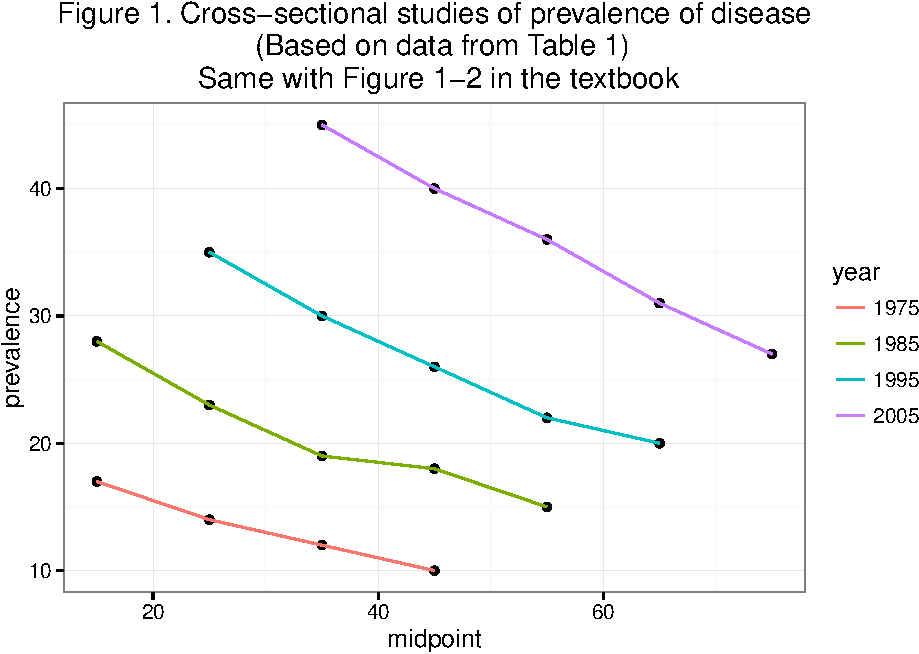
\includegraphics{guidance_files/figure-latex/unnamed-chunk-3-1.pdf}

\subsection{Figure 2
各出生コホートにおいて,縦断的な年齢効果の可視化グラフ (Longitudinal
effect of age for each birth
cohort)}\label{figure-2--longitudinal-effect-of-age-for-each-birth-cohort}

\begin{itemize}
\tightlist
\item
  点線したのは,各出生コホートが加齢している(エージング)時の罹患率を示している.\\
\item
  すべての出生コホートにおいて,加齢とともに,罹患率は増加している.
\end{itemize}

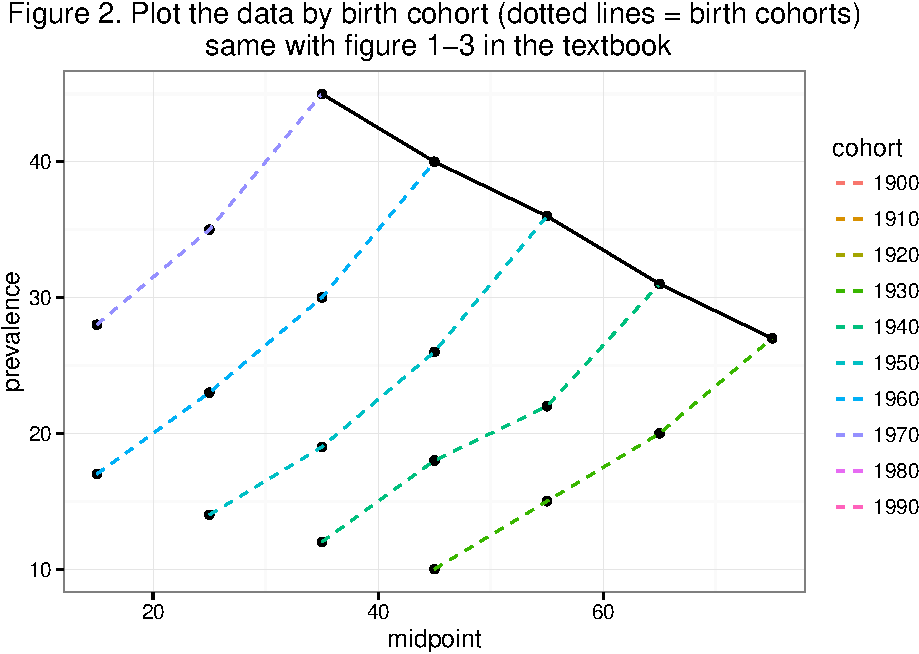
\includegraphics{guidance_files/figure-latex/unnamed-chunk-4-1.pdf}

\subsection{Table 2.
出生コホートによる罹患率を再整理した表}\label{table-2.-}

\begin{itemize}
\tightlist
\item
  出生コホート(横方向)が加齢する時の罹患率は上昇している.
\end{itemize}

\% Table created by stargazer v.5.2 by Marek Hlavac, Harvard University.
E-mail: hlavac at fas.harvard.edu \% Date and time: Wed, Jun 22, 2016 -
11:39:30 AM

\begin{table}[!htbp] \centering 
  \caption{Same with Page 8 Table 1-3 in the textbook} 
  \label{} 
\begin{tabular}{@{\extracolsep{5pt}} cccccccc} 
\\[-1.8ex]\hline 
\hline \\[-1.8ex] 
 & 15 & 25 & 35 & 45 & 55 & 65 & 75 \\ 
\hline \\[-1.8ex] 
1900 & $$ & $$ & $$ & $$ & $$ & $$ & $$ \\ 
1910 & $$ & $$ & $$ & $$ & $$ & $$ & $$ \\ 
1920 & $$ & $$ & $$ & $$ & $$ & $$ & $$ \\ 
1930 & $$ & $$ & $$ & $10$ & $15$ & $20$ & $27$ \\ 
1940 & $$ & $$ & $12$ & $18$ & $22$ & $31$ & $$ \\ 
1950 & $$ & $14$ & $19$ & $26$ & $36$ & $$ & $$ \\ 
1960 & $17$ & $23$ & $30$ & $40$ & $$ & $$ & $$ \\ 
1970 & $28$ & $35$ & $45$ & $$ & $$ & $$ & $$ \\ 
1980 & $$ & $$ & $$ & $$ & $$ & $$ & $$ \\ 
1990 & $$ & $$ & $$ & $$ & $$ & $$ & $$ \\ 
\hline \\[-1.8ex] 
\end{tabular} 
\end{table}

\subsection{Figure 3:}\label{figure-3}

This graph is useful in detecting an unusual birth cohort. If there is a
spike, that specific birth cohort more severely affected than other
cohorts.

This is grouped by the age at the surveys. In each age group, those who
were born more recently (more right) have higher prevalence, i.e., at
the same age, those who were born more recently had higher prevalences
of this hypothetical disease.

\begin{Shaded}
\begin{Highlighting}[]
\NormalTok{## Change age midpoint to categorical}
\NormalTok{tab1}\FloatTok{.2}\NormalTok{.melt$midpoint <-}\StringTok{ }\KeywordTok{factor}\NormalTok{(tab1}\FloatTok{.2}\NormalTok{.melt$midpoint)}

\NormalTok{## Configure prevalence vs birth cohort plot}
\NormalTok{plot.prev.cohort <-}
\StringTok{    }\KeywordTok{ggplot}\NormalTok{(}\DataTypeTok{data =} \KeywordTok{subset}\NormalTok{(tab1}\FloatTok{.2}\NormalTok{.melt, !}\KeywordTok{is.na}\NormalTok{(prevalence)),}
                 \DataTypeTok{mapping =} \KeywordTok{aes_string}\NormalTok{(}\DataTypeTok{x =} \StringTok{"cohort"}\NormalTok{, }
                                      \DataTypeTok{y =} \StringTok{"prevalence"}\NormalTok{)) +}
\StringTok{    }\KeywordTok{geom_point}\NormalTok{() +}
\StringTok{    }\KeywordTok{theme_bw}\NormalTok{() +}
\StringTok{    }\KeywordTok{theme}\NormalTok{(}\DataTypeTok{legend.key =} \KeywordTok{element_blank}\NormalTok{())}

\NormalTok{## Plot grouping by age midpoints}
\NormalTok{fig1}\FloatTok{.4} \NormalTok{<-}\StringTok{ }\NormalTok{plot.prev.cohort +}
\StringTok{  }\KeywordTok{geom_line}\NormalTok{(}\DataTypeTok{mapping =} \KeywordTok{aes_string}\NormalTok{(}\DataTypeTok{group =} \StringTok{"midpoint"}\NormalTok{, }
                                 \DataTypeTok{color =} \StringTok{"midpoint"}\NormalTok{), }\DataTypeTok{lty =} \DecValTok{4}\NormalTok{)}
\NormalTok{fig1}\FloatTok{.4}
\end{Highlighting}
\end{Shaded}

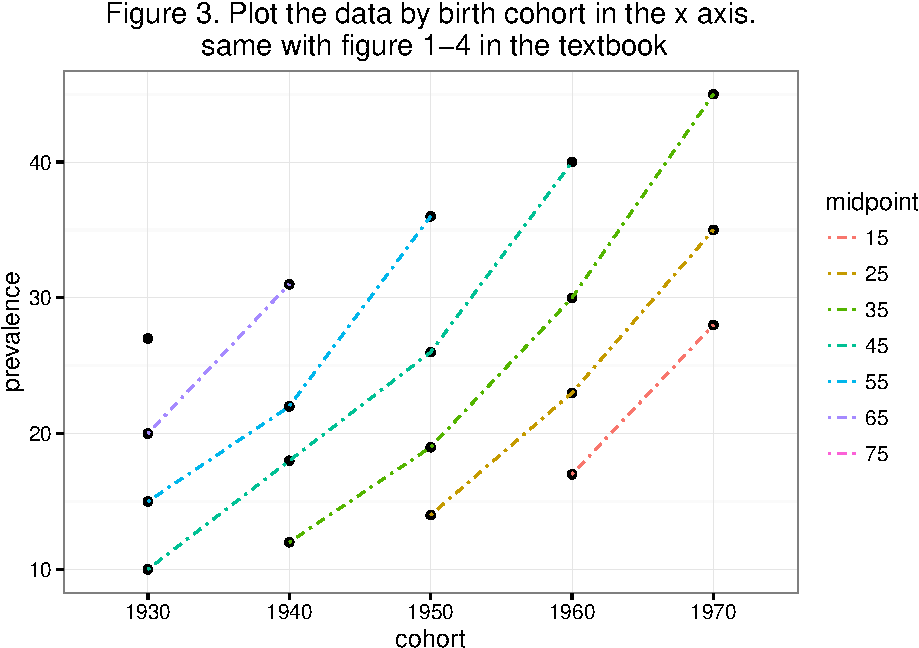
\includegraphics{guidance_files/figure-latex/unnamed-chunk-6-1.pdf}

\section*{参考文献}
\addcontentsline{toc}{section}{参考文献}

\hypertarget{refs}{}
\hypertarget{ref-szkloux5fepidemiology:ux5f2012}{}
{[}1{]} Szklo, M. and Nieto, J. (2012) Epidemiology: Beyond the Basics.
3 edition. Jones \& Bartlett Learning, Burlington, Mass.

\hypertarget{ref-rikan}{}
{[}2{]} 集計表のダウンロード|がん登録・統計[がん情報サービス]
{[}Internet{]}.

\end{document}
